\section{Zusammenfassung}

\begin{concept}{Iterativ-Inkrementeller Entwicklungsprozess}\\
Der Softwareentwicklungsprozess in SWEN1/PM3:
\begin{itemize}
    \item \textbf{Iterationen:}
    \begin{itemize}
        \item 2-Wochen-Rhythmus
        \item Definierte Ziele pro Iteration
        \item Review nach Abschluss
    \end{itemize}
    \item \textbf{Meilensteine:}
    \begin{itemize}
        \item M1: Projektskizze
        \item M2: Lösungsarchitektur
        \item M3: Beta-Release
    \end{itemize}
    \item \textbf{Pro Iteration:}
    \begin{itemize}
        \item Anforderungsanalyse
        \item Design
        \item Implementation
        \item Testing
    \end{itemize}
\end{itemize}
\end{concept}

\begin{theorem}{Zentrale Artefakte}\\
Die wichtigsten Ergebnisse im Entwicklungsprozess:
\begin{itemize}
    \item \textbf{Anforderungsanalyse:}
    \begin{itemize}
        \item Funktionale Anforderungen (Use Cases)
        \item Qualitätsanforderungen und Randbedingungen
        \item Domänenmodell
    \end{itemize}
    \item \textbf{Design:}
    \begin{itemize}
        \item Softwarearchitektur
        \item Use Case Realisierung
        \item Statische und dynamische Modelle
    \end{itemize}
    \item \textbf{Implementation:}
    \begin{itemize}
        \item Quellcode mit Javadoc
        \item Refactoring bei Code Smells
    \end{itemize}
    \item \textbf{Testing:}
    \begin{itemize}
        \item Unit-Tests
        \item Integrationstests
        \item Systemtests
    \end{itemize}
\end{itemize}
\end{theorem}

\begin{concept}{UML in der Praxis}\\
Nach Martin Fowler gibt es drei Haupteinsatzarten:
\begin{itemize}
    \item \textbf{UML as a Sketch:}
    \begin{itemize}
        \item Informelle Diagramme
        \item Kommunikationswerkzeug
        \item Bevorzugt in agiler Entwicklung
    \end{itemize}
    \item \textbf{UML as a Blueprint:}
    \begin{itemize}
        \item Detaillierte Analyse/Design
        \item Code-Generierung
        \item Reverse-Engineering
    \end{itemize}
    \item \textbf{UML as a Programming Language:}
    \begin{itemize}
        \item Ausführbare Spezifikation
        \item MDA-Werkzeuge
    \end{itemize}
\end{itemize}
\end{concept}

\begin{concept}{Objektorientierte Analyse (OOA)}\\
Zentrale Aktivitäten der Anforderungsanalyse:
\begin{itemize}
    \item \textbf{User Research:}
    \begin{itemize}
        \item Personas entwickeln
        \item Contextual Inquiry durchführen
        \item Prototyping und Sketching
    \end{itemize}
    \item \textbf{Use Cases:}
    \begin{itemize}
        \item Modellierung und Dokumentation
        \item UML-Use-Case-Diagramme
        \item UI-Sketching
    \end{itemize}
    \item \textbf{Domänenmodellierung:}
    \begin{itemize}
        \item Konzeptuelles Klassenmodell
        \item Fachbegriffe und Beziehungen
        \item Problembezogene Sicht
    \end{itemize}
\end{itemize}
\end{concept}

\begin{concept}{Objektorientiertes Design (OOD)}\\
Zentrale Design-Aktivitäten:
\begin{itemize}
    \item \textbf{Architektur:}
    \begin{itemize}
        \item UML-Paketdiagramm
        \item UML-Verteilungsdiagramm
    \end{itemize}
    \item \textbf{Use-Case Realisierung:}
    \begin{itemize}
        \item Klassendesign mit Verantwortlichkeiten
        \item Statische Modelle (Klassendiagramm)
        \item Dynamische Modelle (Sequenz-, Zustands-, Aktivitätsdiagramme)
    \end{itemize}
    \item \textbf{Design Patterns:}
    \begin{itemize}
        \item GRASP Prinzipien
        \item GoF Patterns
        \item Architektur Patterns
    \end{itemize}
\end{itemize}
\end{concept}

\begin{concept}{Implementation und Testing}\\
\textbf{Implementation:}
\begin{itemize}
    \item Umsetzung des OO-Designs in Code
    \item Algorithmen und Datenstrukturen
    \item Kontinuierliches Refactoring
    \item Clean Code Prinzipien
\end{itemize}
\textbf{Testing:}
\begin{itemize}
    \item Test-Driven Development
    \item Verschiedene Teststufen
    \item Testkonzept und -dokumentation
\end{itemize}
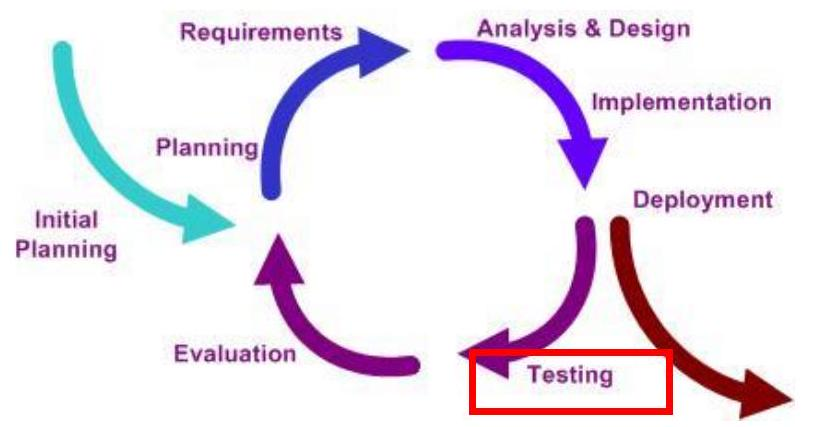
\includegraphics[width=0.8\linewidth]{images/2025_01_02_6eafa38dd4ae10c9a392g-15}
\end{concept}